\section{Neural Network Training}
\label{sec:NeuralNetworks}

\subsection{Coding environment}
\label{sec:CodingEnvironment}

The toy data code example~\cite{AGlazovCode} uses Jupiter Notebook. The ML commands can be run either from Jupiter Notebook or from a regular Python script from a laptop with Anaconda with Python2 or Python3. For this problem, one needs the ability to run \texttt{ROOT} in the same environment to read the \texttt{.root} file with the jet data from the analysis. ROOT can not be run from Anaconda, however. One option is to split the code into two separate files, each run in separate environments and communicating to each other via numpy arrays. This is not ideal, however, since optimising a NN requires many steps. One needs the ability to have all code in one environment and run it all at once.

\ \\Another option is to run the Jupiter Notebook in the server provided by ATLAS called SWAN~\cite{SWAN}. This environment has access to both Keras and ROOT at the same time. Although all commands can be run at once, the server would often die while running due either to bad wifi connection, or due to CERN server being busy.

\ \\To run effectively, it is better to run from only one Python script, instead of from one Jupiter Notebook. The recommended solution is to run from CERN's lxplus machines. Right after the \texttt{ssh}, a \texttt{singularity}~\cite{singularity} ennviroment is set up via a \texttt{docker} container that contains the ML sofware. While \texttt{ROOT} is not contained, the \texttt{uproot}~\cite{uproot} library is included. \texttt{uproot} allows to read the \texttt{.root} files in numpy arrays, the data types that are used natively by the ML libraries such as \texttt{TensorFlow} inside \texttt{Python}. It is this setup that is found to be the most efficient and is used in this project.

\subsection{k-fold}
\label{sec:k-fold}

NN training requires that the data is split in two independent sets. Some is used to train the NN, while the other is used for testing (also called validation). In this project half of the data (the events with even index) is used in training, and the other half of the data (the events with odd index) is used in testing. Since the data is split in two, it is said to have a k-fold=2. It is the simplest case and is what is used in this report.

\ \\Since there are 43076 events, there are 21538 events in training and also 21538 in testing. Each event has a collection of jets, from which the leading jet in \pt~is used for both the reco (input) and truth (output).

\ \\Other possibilities involve having a k larger than 2, for example 5. In that case, the data is split into 5 independent parts. The training and testing contain 5 consecutive steps. One trains in 4 parts and tests in 1, then repeats with another 1 until the data is evaluated once in each event.

\subsection{Neural network overview}
\label{sec:NeuralNetworkOverview}

In machine learning (ML) a solution for a problem is found without being explicitly programmed. The two main classes of ML are supervised and unsupervised. In this project supervised learning is used, as the output is known and is labeled. The machine learning method tries to learn what the labels are as a function of the input.

\ \\Several machine learning algorithms can be used to perform the classification task. In this project neural networks~\cite{AndrewNg} are used. In general, to find a multidimensional highly non-linear function, it is efficient to train a NN. The NN algorithm is inspired from the brain structure and functions. The brain contains millions of neuron cells forming a network where electro-chemical impulses are being passed between them. An artificial neural network is formed by a number of interconnected artificial \emph{neurons}, or \emph{nodes} respects this architecture.

\ \\A neural network is formed by several layers, each containing several nodes. The number of nodes on the first (input) and last (output) layers are fixed by the problem to solve. They are 1 and 25, respectively, for the problem presented in this project. The layers in between are called hidden layers. Their number and the number of their nodes can be optimised for hte particular problem. If there is one hidden layer, the NN is said to be \emph{shallow}. If there are more than one hidden layer, the NN is said to be \emph{deep}. If each node is connected to all nodes of the layer before and after, the NN is said to be fully connected. A general structure of a fully connected deep NN (DNN) is presented in Figure~\ref{fig:DNN}.

\begin{figure}[h]
  \centering
  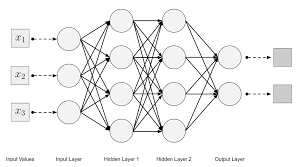
\includegraphics[width=0.6\textwidth]{./plots/DNNArchitecture.png}
  \caption{Diagram of a general architecture of a DNN. Credit image: O'Reilly.~\cite{OReilly}.}
  \label{fig:DNN}
\end{figure}

\ \\The \emph{Universal Approximation Theorem} states that a neural network with one \emph{hidden layer} can in principle approximate any N-dimensional function to an arbitrary degree of accuracy, given a sufficiently large (though finite) number of nodes. In practice however it is more suitable to use multiple hidden layers connected in series~\cite{AndrewNg}.

\ \\In a fully connected NN, each node takes a weighted linear combination of the outputs from nodes of the previous layer, adds its own bias values, and applies an \emph{activation function}, then outputs the result to the nerons of the next layer, as illustrated in Figure~\ref{fig:Neuron}. The activation function is choosen via optimisation for each neuron when the architecture of the NN is defined. 

\begin{figure}[h]
  \centering
  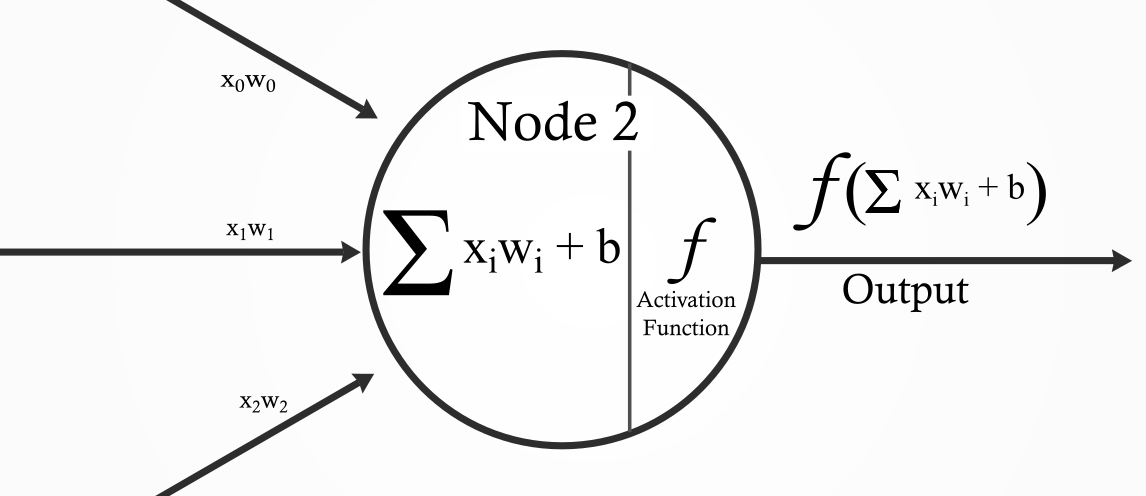
\includegraphics[width=0.6\textwidth]{./plots/Neuron.png}
  \caption{Diagram of a neuron or node in a NN, with its weight inputs, its bias and the output via the activation function. Credit image: The Fork~\cite{TheFork}.}
  \label{fig:Neuron}
\end{figure}

\ \\Once the NN architecture is set the layers, nodes and activation functions, the total function of the NN is parametrized by all the weights for the connections between nodes plus the biases of each node. Training the NN means learning these weights so that the NN function can predict well the output when a new data not seen before is taken as input.

\ \\NN training is done learning on the training dataset and testing on the testing dataset. Running once over all the data from training and testing represents an \emph{epoch}. During an epoch, events are analysed in groups called \emph{batches}. The number of epochs to run on and the number of events in each batch can be optimised.

\ \\ Let's take a look at how the NN training happens. At first the NN has random values for the weights and biases. For each of the events in the first batch, data comes in, and the NN predicts an output values, that are at first very different from the true desired output value. To evaluate how far away are the predicted output from the desired output, a \emph{loss} function is defined that can be chosen from several formulas, but have the generic form of a sum over the absolute values of these differences. The goal of the NN training is to update the values of the weights and biases so that the loss function is minimized. After the first batch, the NN changes the weights via a back-propagation aglorithm that can be selected from several, and usually it is a form of gradiant descent. For each new batch, the weights and biases change, and become continously closer to the correct values, as the loss function becomes gradually smaller. When all the training events are used, the first epoch is finished. The NN function at this point is then applied to the new dataset from the testing dataset, which is not split in batches, and a loss function is also calculated. The entire procedure repeats for the number of epochs chosen. At the end, the final weights and biases define the final NN that has been learned.

\ \\There is also another figure of merit of how well does a NN perform in training and testing. It is called \emph{accuracy} and is related to the number of of true positives or false negatives. The larger the accuracy, the better.

\ \\For the training dataset, the loss and accuracy values always improve. But in the testing dataset they can start to degrade if we train for too many epochs. By degrading it means that the loss value starts to grow, and the accuracy value starts to decrease. That is called over-training and consists of memorizing the inputs, and thus not being able to predict correctly any more for new inputs. 

\subsection{Neural network optimisation}
\label{sec:NeuralNetworkOptimisation}

An optimisation of the NN training hyper-parameters described in the Section~\ref{sec:NeuralNetworkOverview} is made by changing only one at a time, while keeping the other constant. The best choice is the one with largest accuracy and smallest loss values. The best of the studied NNs is denoted as the new NN. It is a deep NN. The NN from the code example is denoted as the old NN. It is a shallow NN. Figure~\ref{fig:NNArchitecture} visualises the architectures and activation functions of the old NN (top) and the new NN (bottom).

\begin{figure}[h]
  \centering
  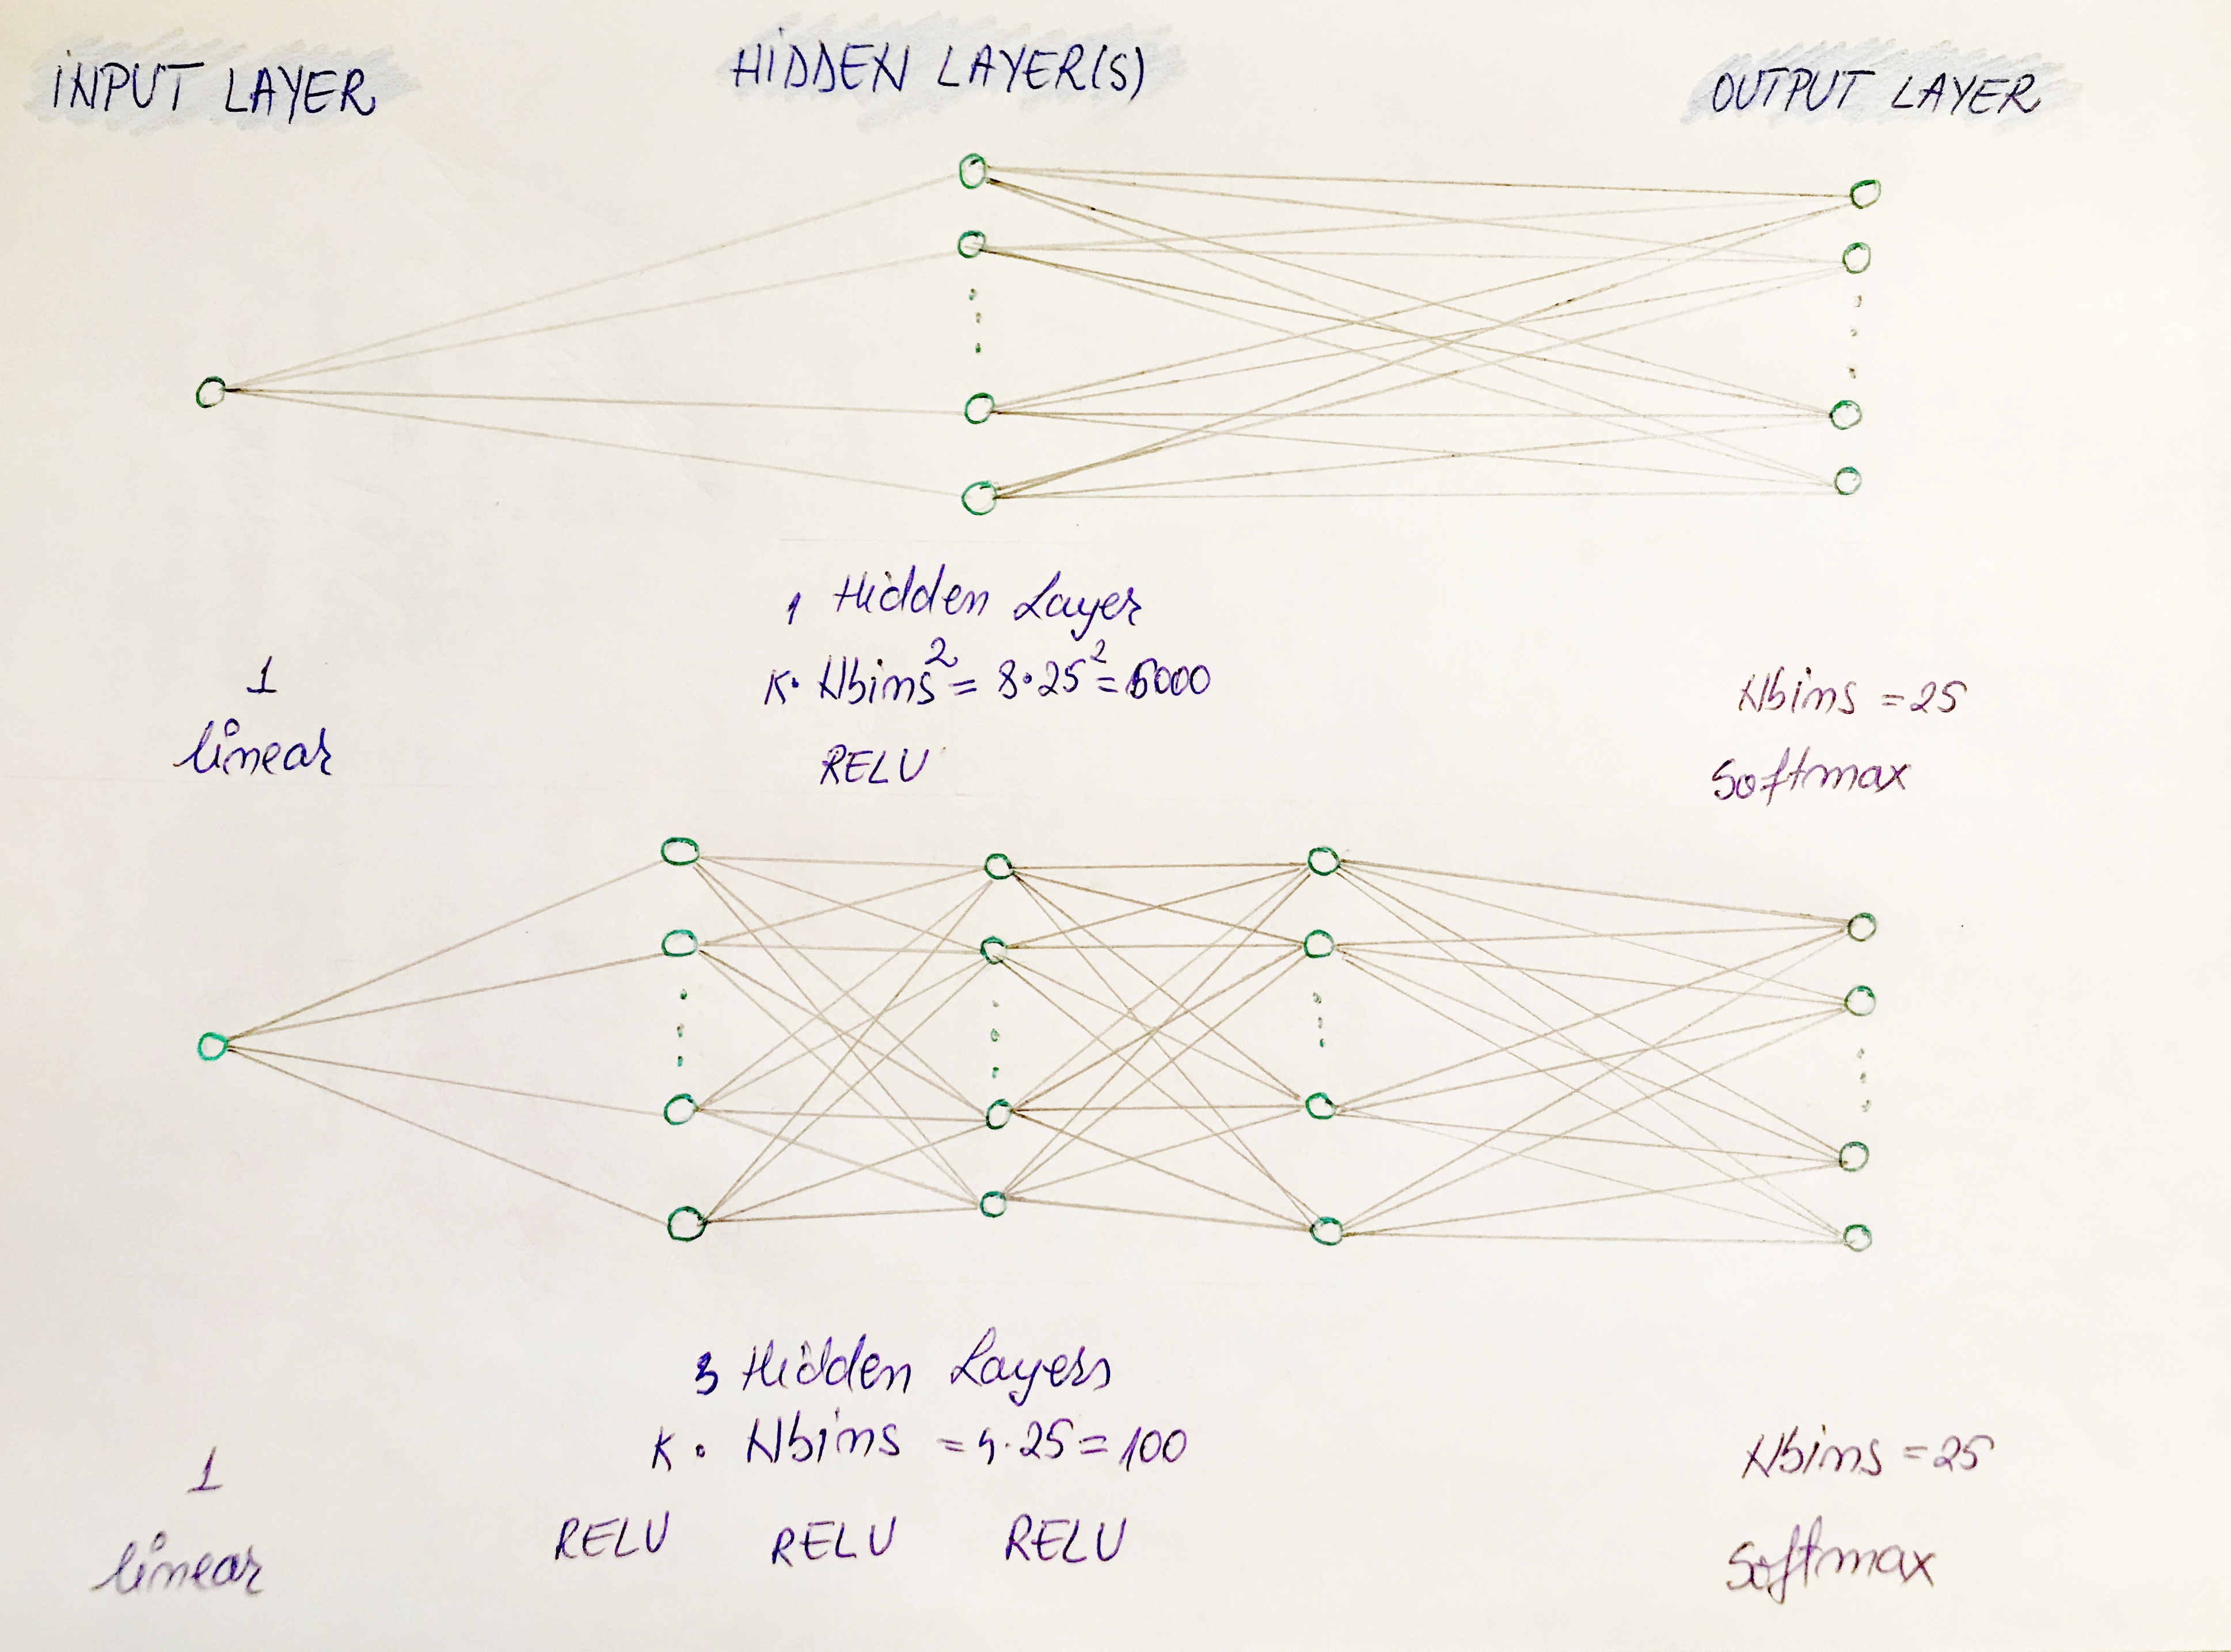
\includegraphics[width=0.9\textwidth]{../presentation/plots/NNArchitecture.jpg}
  \caption{NN architectures and activation functions for the old and shallow NN (top) and the new and deep NN (bottom).}
  \label{fig:NNArchitecture}
\end{figure} 

\ \\The input and output layers are the same, constrained by the physics problem to solve. The input layer has only one node and uses the \emph{linear} activation function. It means the input data is passed out from the first neuron. The output layer has 25 output variables. It uses the \emph{softmax} activation function~\cite{softmax}, which ensures that the output of each node is a number between 0 and 1 and the sum of all these numbers is exactly 1. This ensures that the value of each node is interpreted as the probability that the jet falls in the bin index represented by that node.

\ \\The hidden layers have differences. The old NN has only one layer with very many nodes. The new NN has three layers, each with fewer nodes. Both NN use the same \emph{ReLU} activation function~\cite{ReLU}. ReLU is the recommended modern activation function to use as default when starting to study a new problem. The ReLu activation function is zero for negative values and the diagonal for positive values, as seen in Figure~\ref{fig:ReLU}. In future developments of the project, more complex activation functions can be used.

\begin{figure}[h]
  \centering
  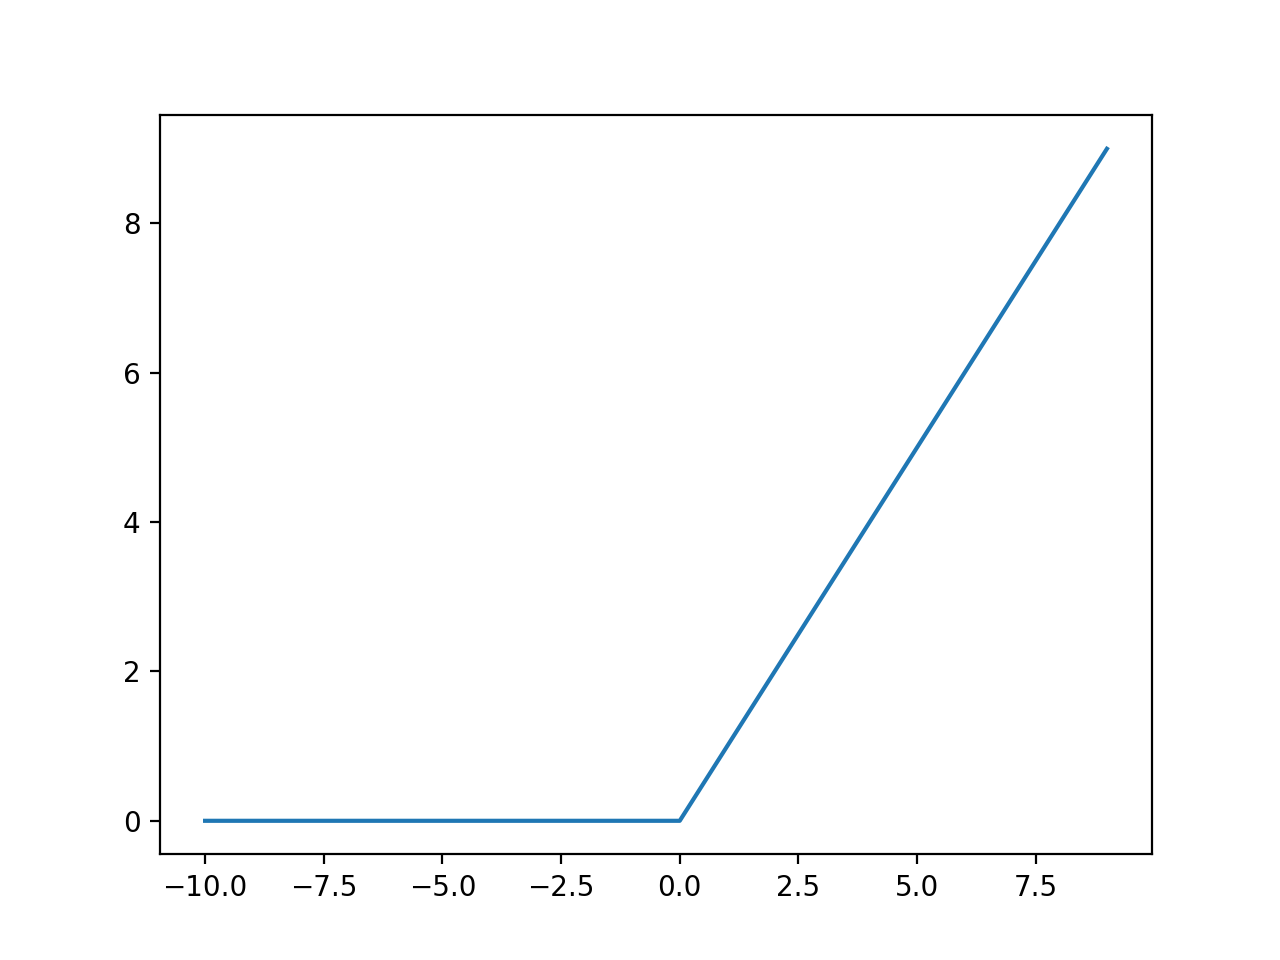
\includegraphics[width=0.5\textwidth]{./plots/ReLU.png}
  \caption{The ReLu activation function is zero for negative values and the diagonal for positive values~\cite{ReLU}.}
  \label{fig:ReLU}
\end{figure} 

\ \\The possible choices in hyper-parameters comparing the old and the new NN are summarised in Table~\ref{tab:NNOldNew}.

\begin{table}[h!]
  \resizebox{\textwidth}{!}{
    \begin{tabular}{|l|l|l|} % <-- Alignments: 1st column left, 2nd middle and 3rd right, with vertical lines in between
      \hline
      \textbf{Choice} & \textbf{Old NN (toy data example)} & \textbf{New NN (my best choice)}\\
      \hline
      number of nodes per input layer & 1 & 1 \\
      number of nodes per output layer & ${\rm Nbins}=25$ & ${\rm Nbins}=25$ \\
      Number of hidden layers & 1 & 3 \\
      ${\rm k}$ & 8 & 4 \\
      Number of nodes per layer & ${\rm k}\cdot {\rm Nbins}^2=5000$ & ${\rm k}\cdot {\rm Nbins}=100$ \\
      activation function input & linear & linear \\
      activation function hidden & ReLU & ReLU \\
      activation function output & softmax & softmax \\
      batch size & 1000 & 200 \\
      number of epochs & 150 & 150 \\
      \hline
    \end{tabular}
  }
\caption {NN architecture and hyper-parameters comparing for the old NN, suggested in the toy data paper, and the new NN, from the optimisation of this study.}
\label{tab:NNOldNew}
\end{table}

\ \\Figure~\ref{fig:accuracylossTrainTest} shows the overlay of train and test for the two figures of merit (accuracy and loss). The train and test curves are very similar. This confirms that the NNs are not overtrained. Figure~\ref{fig:accuracylossOldNew} shows the overlay of the old and the new NNs for the two figures of merit. For the accuracy, the larger the better. For the loss, the smaller the better. The new NN is better than the old NN for both figures of merit. 

\begin{figure}[t]
  \centering
  \includegraphics[width=0.45\textwidth]{../output_20GeV/NN_plot1D_optionTrainTest_accuracy_NN_l_A1_k_8_e_150_b_1000.pdf}
  \includegraphics[width=0.45\textwidth]{../output_20GeV/NN_plot1D_optionTrainTest_accuracy_NN_l_B3_k_4_e_150_b_200.pdf}\\
  \includegraphics[width=0.45\textwidth]{../output_20GeV/NN_plot1D_optionTrainTest_loss_NN_l_A1_k_8_e_150_b_1000.pdf}
  \includegraphics[width=0.45\textwidth]{../output_20GeV/NN_plot1D_optionTrainTest_loss_NN_l_B3_k_4_e_150_b_200.pdf}
  \caption{Overlay of train and test for the accuracy (top) and loss (bottom). Old NN (left) and new NN (right).}
  \label{fig:accuracylossTrainTest}
\end{figure}

\begin{figure}[b]
  \centering
  \includegraphics[width=0.45\textwidth]{../output_20GeV/NN_plot1D_train_accuracy_NN_final.pdf}
  \includegraphics[width=0.45\textwidth]{../output_20GeV/NN_plot1D_test_accuracy_NN_final.pdf}\\
  \includegraphics[width=0.45\textwidth]{../output_20GeV/NN_plot1D_train_loss_NN_final.pdf}
  \includegraphics[width=0.45\textwidth]{../output_20GeV/NN_plot1D_test_loss_NN_final.pdf}
  \caption{Overlay with old and new NN for the accuracy (top) and loss (bottom). Train (left) and test (right).}
  \label{fig:accuracylossOldNew}
\end{figure}
